\documentclass[journal,12pt,twocolumn]{IEEEtran}

\usepackage{setspace}
\usepackage{gensymb}
\singlespacing
\usepackage[cmex10]{amsmath}

\usepackage{amsthm}

\usepackage{mathrsfs}
\usepackage{txfonts}
\usepackage{stfloats}
\usepackage{bm}
\usepackage{cite}
\usepackage{cases}
\usepackage{subfig}

\usepackage{longtable}
\usepackage{multirow}

\usepackage{enumitem}
\usepackage{mathtools}
\usepackage{steinmetz}
\usepackage{tikz}
\usepackage{circuitikz}
\usepackage{verbatim}
\usepackage{tfrupee}
\usepackage[breaklinks=true]{hyperref}
\usepackage{graphicx}
\usepackage{tkz-euclide}
\usepackage{float}

\usetikzlibrary{calc,math}
\usepackage{listings}
    \usepackage{color}                                            %%
    \usepackage{array}                                            %%
    \usepackage{longtable}                                        %%
    \usepackage{calc}                                             %%
    \usepackage{multirow}                                         %%
    \usepackage{hhline}                                           %%
    \usepackage{ifthen}                                           %%
    \usepackage{lscape}     
\usepackage{multicol}
\usepackage{chngcntr}

\DeclareMathOperator*{\Res}{Res}
\newtheorem{theorem}{Theorem}[section]
\newtheorem{corollary}{Corollary}[theorem]
\newtheorem{lemma}[theorem]{Lemma}
\newtheorem{definition}{Definition}[section]
\renewcommand\thesection{\arabic{section}}
\renewcommand\thesubsection{\thesection.\arabic{subsection}}
\renewcommand\thesubsubsection{\thesubsection.\arabic{subsubsection}}

\renewcommand\thesectiondis{\arabic{section}}
\renewcommand\thesubsectiondis{\thesectiondis.\arabic{subsection}}
\renewcommand\thesubsubsectiondis{\thesubsectiondis.\arabic{subsubsection}}


\hyphenation{op-tical net-works semi-conduc-tor}
\def\inputGnumericTable{}                                 %%

\lstset{
%language=C,
frame=single, 
breaklines=true,
columns=fullflexible
}
\begin{document}

\newcommand{\BEQA}{\begin{eqnarray}}
\newcommand{\EEQA}{\end{eqnarray}}
\newcommand{\define}{\stackrel{\triangle}{=}}
\bibliographystyle{IEEEtran}
\raggedbottom
\setlength{\parindent}{0pt}
\providecommand{\mbf}{\mathbf}
\providecommand{\pr}[1]{\ensuremath{\Pr\left(#1\right)}}
\providecommand{\qfunc}[1]{\ensuremath{Q\left(#1\right)}}
\providecommand{\sbrak}[1]{\ensuremath{{}\left[#1\right]}}
\providecommand{\lsbrak}[1]{\ensuremath{{}\left[#1\right.}}
\providecommand{\rsbrak}[1]{\ensuremath{{}\left.#1\right]}}
\providecommand{\brak}[1]{\ensuremath{\left(#1\right)}}
\providecommand{\lbrak}[1]{\ensuremath{\left(#1\right.}}
\providecommand{\rbrak}[1]{\ensuremath{\left.#1\right)}}
\providecommand{\cbrak}[1]{\ensuremath{\left\{#1\right\}}}
\providecommand{\lcbrak}[1]{\ensuremath{\left\{#1\right.}}
\providecommand{\rcbrak}[1]{\ensuremath{\left.#1\right\}}}
\theoremstyle{remark}
\newtheorem{rem}{Remark}
\newtheorem*{remark}{Remark}
\newcommand{\sgn}{\mathop{\mathrm{sgn}}}
\providecommand{\abs}[1]{\vert#1\vert}
\providecommand{\res}[1]{\Res\displaylimits_{#1}} 
\providecommand{\norm}[1]{\lVert#1\rVert}
%\providecommand{\norm}[1]{\lVert#1\rVert}
\providecommand{\mtx}[1]{\mathbf{#1}}
\providecommand{\mean}[1]{E[ #1 ]}
\providecommand{\fourier}{\overset{\mathcal{F}}{ \rightleftharpoons}}
%\providecommand{\hilbert}{\overset{\mathcal{H}}{ \rightleftharpoons}}
\providecommand{\system}{\overset{\mathcal{H}}{ \longleftrightarrow}}
	%\newcommand{\solution}[2]{\textbf{Solution:}{#1}}
\newcommand{\solution}{\noindent \textbf{Solution: }}
\newcommand{\cosec}{\,\text{cosec}\,}
\providecommand{\dec}[2]{\ensuremath{\overset{#1}{\underset{#2}{\gtrless}}}}
\newcommand{\myvec}[1]{\ensuremath{\begin{pmatrix}#1\end{pmatrix}}}
\newcommand{\mydet}[1]{\ensuremath{\begin{vmatrix}#1\end{vmatrix}}}
\numberwithin{equation}{subsection}
\makeatletter
\@addtoreset{figure}{problem}
\makeatother
\let\StandardTheFigure\thefigure
\let\vec\mathbf
\renewcommand{\thefigure}{\theproblem}
\def\putbox#1#2#3{\makebox[0in][l]{\makebox[#1][l]{}\raisebox{\baselineskip}[0in][0in]{\raisebox{#2}[0in][0in]{#3}}}}
     \def\rightbox#1{\makebox[0in][r]{#1}}
     \def\centbox#1{\makebox[0in]{#1}}
     \def\topbox#1{\raisebox{-\baselineskip}[0in][0in]{#1}}
     \def\midbox#1{\raisebox{-0.5\baselineskip}[0in][0in]{#1}}
\vspace{3cm}
\title{EE3900 - Gate Assignment 2}
\author{W Vaishnavi - AI20BTECH11025}
\maketitle
\newpage
\bigskip
\renewcommand{\thefigure}{\theenumi}
\renewcommand{\thetable}{\theenumi}
Download all latex-tikz codes from 
%
\begin{lstlisting}
https://github.com/vaishnavi-w/EE3900/blob/main/Gate2/latex2.tex
\end{lstlisting}
and python codes from 
%
\begin{lstlisting}
https://github.com/vaishnavi-w/EE3900/blob/main/Gate2/codes
\end{lstlisting}
\section{Gate EC - 2005}
Choose the function $f\brak{t} ; -\infty < t < \infty$ for which a fourier series cannot be defined
\begin{enumerate}[label=\Alph*)]
    \item $3\sin\brak{25t}$
    \item $4\cos{\brak{20t+3}} + 2\sin{\brak{10t}}$
    \item $exp\brak{-|t|}\sin{\brak{25t}}$
    \item 1
\end{enumerate}
\section{Solution}
Fourier series is defined for periodic or constant functions
\begin{enumerate}
    \item $f(t) = 3\sin\brak{25t}$\\
    The given signal is sinusoidal with time period 
    \begin{align}
        T = \frac{2\pi}{25}
    \end{align}
    Hence, fourier series can be defined.
    \begin{figure}[H]
    \centering
    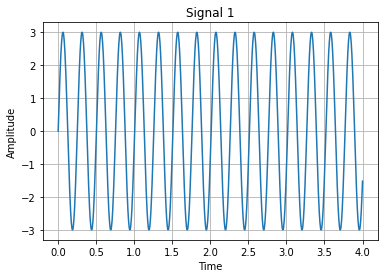
\includegraphics[width=\columnwidth]{signal1.png}
    \caption{Plot of Signal 1}
    \label{fig:signal_1}
    \end{figure}
    \item $f(t) = 4\cos{\brak{20t+3}} + 2\sin{\brak{10t}}$\\
    The given signal is the sum of two periodic signals with time periods $T_1, T_2$
    \begin{align}
        T_1 = \frac{2\pi}{20}\\
        T_2 = \frac{2\pi}{10}
    \end{align}
    Sum of two periodic signals is periodic if the ratio of their periods is rational
    \begin{align}
        \frac{T_1}{T_2} = \frac{2\pi/20}{2\pi/10} = \frac{1}{2}
    \end{align}
    Thus, the given signal is periodic and fourier series can be defined.
    \begin{figure}[H]
    \centering
    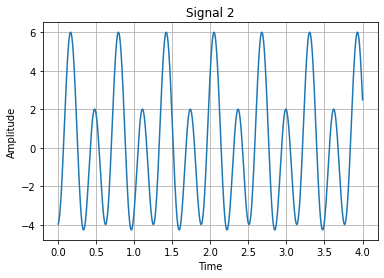
\includegraphics[width=\columnwidth]{signal2.png}
    \caption{Plot of Signal 2}
    \label{fig:signal_2}
    \end{figure}
    \item $f(t) = exp\brak{-|t|}\sin{\brak{25t}}$\\
    Due to the decaying exponential function, the signal is not periodic. Fourier series cannot be defined for it.
    \begin{figure}[H]
    \centering
    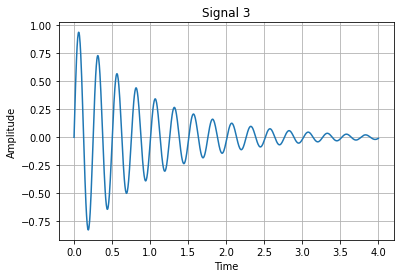
\includegraphics[width=\columnwidth]{signal3.png}
    \caption{Plot of Signal 3}
    \label{fig:signal_3}
    \end{figure}
    \item $f(t) = 1$\\
    It is a constant function. Fourier series can be defined.
\end{enumerate}
\textbf{Answer :} Option C
\end{document}